\documentclass[tikz,border=2pt]{standalone}
\usetikzlibrary{positioning}

\usepackage{anyfontsize} % allows arbitrary font sizes
\usepackage{lmodern} % better font scaling

\makeatletter
\renewcommand\normalsize{%
  \@setfontsize\normalsize{16pt}{19pt}%
}
\renewcommand\Large{%
  \@setfontsize\Large{20pt}{24pt}%
}
\makeatother

\begin{document}

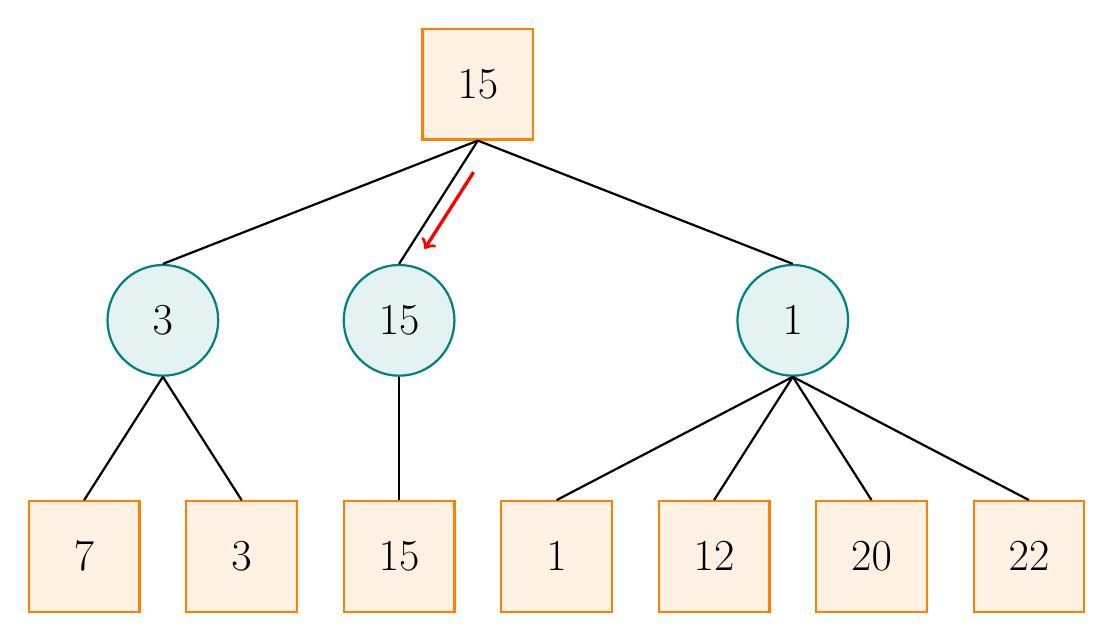
\begin{tikzpicture}[
    xscale=2, yscale=3, thick,
    max node/.style={draw,orange,rectangle,fill=orange!10!white,inner sep=-10pt,minimum size=40pt,text=black},
    min node/.style={draw,teal,circle,fill=teal!10!white,inner sep=-10pt,minimum size=40pt,text=black},
]

\node[max node] (a1)  at (0,0) { $7$ };
\node[max node] (a2)  at (1,0) { $3$ };
\node[max node] (a3)  at (2,0) { $15$ };
\node[max node] (a4)  at (3,0) { $1$ };
\node[max node] (a5)  at (4,0) { $12$ };
\node[max node] (a6)  at (5,0) { $20$ };
\node[max node] (a7)  at (6,0) { $22$ };

\node[min node] (b1) at (0.5,1) { $3$ };
\node[min node] (b2) at (2,1)   { $15$ };
\node[min node] (b3) at (4.5,1) { $1$ };

\node[max node] (c1) at (2.5,2) { $15$ };

\draw (b1.south) -- (a1.north);
\draw (b1.south) -- (a2.north);
\draw (b2.south) -- (a3.north);
\draw (b3.south) -- (a4.north);
\draw (b3.south) -- (a5.north);
\draw (b3.south) -- (a6.north);
\draw (b3.south) -- (a7.north);
\draw (c1.south) -- (b1.north);
\draw (c1.south) -- (b2.north);
\draw (c1.south) -- (b3.north);

\draw[->, red, very thick, shorten >=6mm, shorten <=1mm] 
  ([yshift=-3pt]c1.south) -- ([yshift=-3pt]b2.north);

\end{tikzpicture}

\end{document}
